\documentclass{article}

% Pass numbered, compressed citations to natbib
\PassOptionsToPackage{numbers, compress}{natbib}
% before loading neurips_2026

\usepackage[preprint]{neurips_2026}
% Options:
%  \usepackage[main]{neurips_2026}          % Main Track (double-blind)
%  \usepackage[preprint]{neurips_2026}      % arXiv / preprint
%  \usepackage[main, final]{neurips_2026}   % Camera-ready

\usepackage[utf8]{inputenc} % allow utf-8 input
\usepackage[T1]{fontenc}    % use 8-bit T1 fonts
\usepackage[colorlinks=true,linkcolor={blue!70!black},citecolor={blue!70!black},urlcolor={blue!70!black},hypertexnames=false]{hyperref}
\usepackage{url}            % simple URL typesetting
\usepackage{booktabs}       % professional-quality tables
\usepackage{colortbl}       % \cellcolor in tables
\usepackage{amsfonts}       % blackboard math symbols
\usepackage{nicefrac}       % compact symbols for 1/2, etc.
\usepackage{microtype}      % microtypography
\usepackage{xcolor}         % colors
\usepackage{graphicx}       % includegraphics
\usepackage{subcaption}     % subfigures with (a), (b) labels
\usepackage{amsmath,amssymb,amsthm} % math
\usepackage{algorithm}
\usepackage{algorithmic}
\usepackage{tikz}
\usetikzlibrary{arrows.meta,positioning,calc,decorations.pathreplacing,fit}

% Colors for agent states (Wong colorblind-safe palette)
\definecolor{buyblue}{HTML}{0072B2}
\definecolor{holdgray}{HTML}{AAAAAA}
\definecolor{sellorange}{HTML}{D55E00}
\definecolor{edgegreen}{HTML}{009E73}
\definecolor{lightbg}{HTML}{F0F0F0}

\setcounter{topnumber}{2}
\setcounter{bottomnumber}{1}
\renewcommand{\topfraction}{0.7}

\newtheorem{theorem}{Theorem}
\newtheorem{lemma}[theorem]{Lemma}
\newtheorem{proposition}[theorem]{Proposition}
\newtheorem{corollary}[theorem]{Corollary}
\theoremstyle{definition}
\newtheorem{definition}[theorem]{Definition}
\theoremstyle{remark}
\newtheorem{remark}[theorem]{Remark}

\title{Agent-Based Models of Financial Markets: A Wolfram Perspective\thanks{Repository: \url{https://github.com/varnerlab/Wolfram-markets-abm-paper.git}.}}

\author{%
  Jeffrey D. Varner \\
  R.F. Smith School of Chemical and Biomolecular Engineering\\
  Cornell University, Ithaca, NY 14850 \\
  \texttt{jdv27@cornell.edu} \\
}

\begin{document}

\maketitle

\begin{abstract}
Financial markets crash without proportionate external shocks, yet most agent-based models
either assume global (mean-field) coupling that erases the spatial structure of contagion,
or employ ad hoc behavioral rules that resist systematic analysis. We introduce a minimal
model in which traders on a two-dimensional grid follow deterministic Wolfram totalistic
cellular automaton (CA) rules with three states---Buy, Hold, Sell---and update from their
four cardinal neighbors. Boundary agents inject real market sentiment derived from QQQ ETF
minute-bar data via a Bollinger Band filter; interior agents are governed by one of two
rules, a majority/herding rule and a contrarian/destabilizer rule, whose mixture fraction~$f$
is the single control parameter. The model exhibits a sharp first-order phase transition at
a critical minority fraction $f_c \approx 0.145$: below this threshold the market is stable,
while above it the system abruptly locks into a sell-dominated regime. At the transition,
sell cascades nucleate from localized seeds and propagate as spatially coherent wavefronts,
a contagion mechanism that is invisible to mean-field treatments and that connects naturally
to the tipping-point phenomenology observed in real markets. Because the full rule space
($3^9 = 19{,}683$ rules) is finite and enumerable, the framework enables systematic
screening of agent behaviors---a property unavailable in models with continuous parameters.
\end{abstract}

% ============================================================================
\section{Introduction}
% ============================================================================

Financial markets crash. They crash without proportionate external shocks, without advance
warning from traditional risk metrics, and with a statistical regularity---heavy-tailed
return distributions, volatility clustering, and transient negative
autocorrelation---that is remarkably consistent across instruments, geographic markets,
and sampling frequencies~\cite{cont2001empirical,mandelbrot1963variation,sornette2017why}.
A natural question arises: \emph{what is the minimal microscopic mechanism that is sufficient
to produce these phenomena?} If the answer involves the collective dynamics of interacting
agents rather than exogenous shocks, then the spatial structure of those
interactions---who talks to whom, and how far signals travel---matters at least as much as
the decision rules themselves~\cite{battiston2016complexity}.

The ingredients for an answer already exist, though they have not been assembled. On one
side, a generation of agent-based models (ABMs) has demonstrated that heterogeneous
populations of chartists and fundamentalists can reproduce fat tails and clustered
volatility~\cite{lux1999scaling,bak1997price}, that herding on random graphs is sufficient
to generate power-law-tailed returns~\cite{cont2000herd}, and that minority-game
dynamics~\cite{challet1997minority} and adaptive strategy
switching~\cite{farmer2002price,hommes2006heterogeneous} produce non-Gaussian fluctuations
without any exogenous noise assumption. On the other side, a mature literature on lattice
and spin models---Ising models with market
coupling~\cite{bornholdt2001ising,krawiecki2002volatility}, opinion dynamics on
chains~\cite{sznajd2002simple}, and the three-state speculative model of
Kaizoji~\cite{kaizoji2002speculative}---has shown that nearest-neighbor interactions on a
regular grid can produce phase transitions between ordered (crash) and disordered (efficient)
regimes. Meanwhile, cellular automata (CA) have been applied to financial
markets~\cite{wei2003cellular,qiu2007cellular,yang2019financial}, but only with ad hoc rule
designs that resist systematic comparison. What is missing is a framework that combines
\emph{local} spatial dynamics on a regular lattice with a \emph{complete, enumerable} space
of behavioral rules and a \emph{direct} connection to real market data.

In this paper, we close that gap. We model agent interactions on a two-dimensional grid
governed by Wolfram totalistic CA rules~\cite{wolfram2002new}, in which each agent occupies
one cell, maintains one of three states---Buy, Hold, or Sell---and updates deterministically
from the states of its four cardinal neighbors. The totalistic rule framework provides two
properties that are unavailable in prior financial ABMs: strictly local information
propagation, so that sell cascades must spread from neighbor to neighbor as spatially resolved
wavefronts; and a finite, enumerable rule space ($3^9 = 19{,}683$ rules), enabling systematic
screening of agent behaviors rather than ad hoc rule design. We study two complementary
configurations (Figure~\ref{fig:schematic}). In \textbf{Model~A} (open), boundary agents
observe real QQQ ETF minute-bar data via a Bollinger Band filter, injecting exogenous market
sentiment that validates the CA against empirical time series. In \textbf{Model~B} (closed),
the boundary agents respond to an endogenous price formed from the grid's own net order
imbalance, creating a reflexive feedback loop that produces crashes without any external input.
The single control parameter is the minority (contrarian) agent fraction~$f$, and the central
result is a sharp first-order phase transition at a critical threshold $f_c \approx 0.145$:
below $f_c$ the market is stable; above $f_c$ the system abruptly locks into a sell-dominated
regime. The transition is discontinuous, occurring over $\Delta f < 0.01$, consistent with a
tipping-point mechanism rather than a gradual crossover~\cite{scheffer2009early}. At the
transition, sell cascades nucleate from localized seeds and propagate as coherent spatial
wavefronts---a contagion mechanism that is invisible to mean-field treatments and that
connects naturally to the growing body of work on early-warning signals for critical
transitions in complex systems~\cite{scheffer2009early,battiston2016complexity}.

Section~\ref{sec:related} reviews related work on ABMs, lattice models, and CA in finance.
Section~\ref{sec:background} introduces the CA rule framework and edge-agent decision model.
Section~\ref{sec:methods} describes the simulation procedure for Models~A and~B.
Section~\ref{sec:results} presents the phase diagram and grid dynamics, and
Section~\ref{sec:conclusion} concludes.

% --- Figure 1: Model Schematic ---
\begin{figure}[tb]
\centering
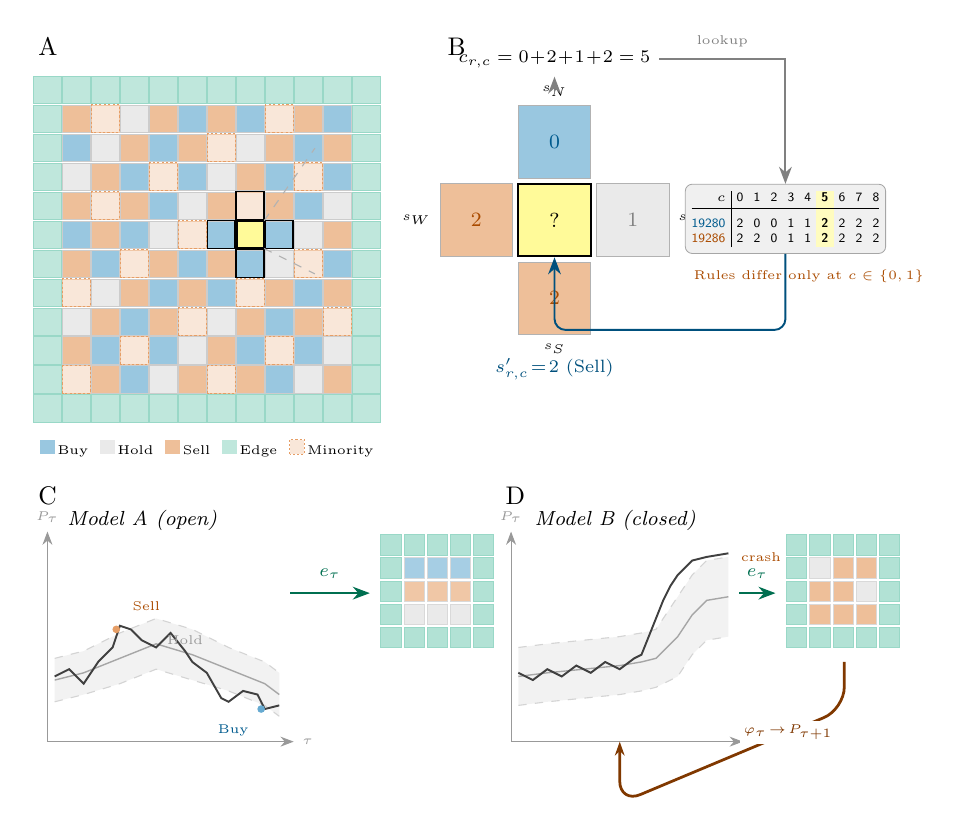
\begin{tikzpicture}[scale=0.92, every node/.style={transform shape},
    >=Stealth,
    annot/.style={font=\scriptsize},
    tinyannot/.style={font=\tiny},
    panellabel/.style={font=\normalsize, anchor=south west},
    % Grid cell styles
    cell/.style={minimum size=3.8mm, draw=black!20, line width=0.15pt, inner sep=0pt},
    edgecell/.style={cell, fill=edgegreen!25, draw=edgegreen!40},
    buycell/.style={cell, fill=buyblue!40},
    holdcell/.style={cell, fill=holdgray!25},
    sellcell/.style={cell, fill=sellorange!40},
    minorcell/.style={cell, fill=sellorange!15, draw=sellorange!35,
                      postaction={draw=sellorange!60, line width=0.3pt,
                      dash pattern=on 0.8pt off 0.8pt}},
    % Zoomed neighborhood
    zcell/.style={minimum size=10mm, draw=black!30, line width=0.35pt, inner sep=0pt,
                  font=\footnotesize},
    % Flow blocks
    fblock/.style={draw=black!50, rounded corners=3pt, minimum height=8mm,
                   font=\footnotesize, fill=white, inner sep=4pt, line width=0.45pt},
    datablock/.style={fblock, fill=buyblue!6, draw=buyblue!40},
    procblock/.style={fblock, fill=lightbg, draw=black!40},
    gridblock/.style={fblock, fill=edgegreen!8, draw=edgegreen!40},
    farrow/.style={->, black!65, line width=0.55pt},
    thickarrow/.style={->, black!50, line width=0.7pt},
]

% =====================================================================
%  ROW 1 — PANEL A (grid) + PANEL B (zoom + rule)
% =====================================================================

% --- Panel A: 12x12 Agent Grid ---
\node[panellabel] at (-0.25, 4.75) {A};

\foreach \r in {0,...,11} {
  \foreach \c in {0,...,11} {
    \pgfmathsetmacro{\xpos}{\c*0.40}
    \pgfmathsetmacro{\ypos}{\r*0.40}
    \ifnum\r=0
      \node[edgecell] (g\r\c) at (\xpos,\ypos) {};
    \else\ifnum\r=11
      \node[edgecell] (g\r\c) at (\xpos,\ypos) {};
    \else\ifnum\c=0
      \node[edgecell] (g\r\c) at (\xpos,\ypos) {};
    \else\ifnum\c=11
      \node[edgecell] (g\r\c) at (\xpos,\ypos) {};
    \else
      \pgfmathparse{int(mod(\r*7+\c*13+3,11))}
      \ifnum\pgfmathresult<2
        \node[minorcell] (g\r\c) at (\xpos,\ypos) {};
      \else
        \pgfmathparse{int(mod(\r*3+\c*7+1,5))}
        \ifnum\pgfmathresult<2
          \node[buycell] (g\r\c) at (\xpos,\ypos) {};
        \else\ifnum\pgfmathresult=2
          \node[holdcell] (g\r\c) at (\xpos,\ypos) {};
        \else
          \node[sellcell] (g\r\c) at (\xpos,\ypos) {};
        \fi\fi
      \fi
    \fi\fi\fi\fi
  }
}

% Highlight target cell (6,7) and Von Neumann neighbors
\node[cell, fill=yellow!40, draw=black, line width=0.8pt] at (7*0.40, 6*0.40) {};
\foreach \dr/\dc in {1/0, -1/0, 0/1, 0/-1} {
  \pgfmathsetmacro{\nr}{int(6+\dr)}
  \pgfmathsetmacro{\nc}{int(7+\dc)}
  \draw[black, line width=0.6pt]
    ($(g\nr\nc.south west)$) rectangle ($(g\nr\nc.north east)$);
}

% Legend row below grid
\node[tinyannot, anchor=north] at (2.2, -0.3) {%
  \begin{tabular}{@{}c@{\,}l@{~~}c@{\,}l@{~~}c@{\,}l@{~~}c@{\,}l@{~~}c@{\,}l@{}}
    \tikz\fill[buyblue!40] (0,0) rectangle (0.2,0.2); & Buy &
    \tikz\fill[holdgray!25] (0,0) rectangle (0.2,0.2); & Hold &
    \tikz\fill[sellorange!40] (0,0) rectangle (0.2,0.2); & Sell &
    \tikz\fill[edgegreen!25] (0,0) rectangle (0.2,0.2); & Edge &
    \tikz\draw[fill=sellorange!15,draw=sellorange!60,line width=0.3pt,
      dash pattern=on 0.8pt off 0.8pt] (0,0) rectangle (0.2,0.2); & Minority \\
  \end{tabular}};

% --- Panel B: Zoomed neighborhood + rule lookup ---
\node[panellabel] at (5.4, 4.75) {B};

% Dashed zoom lines from grid to zoomed cross
\draw[black!30, dashed, line width=0.4pt]
  (g67.north east) -- ++(0.7, 1.0);
\draw[black!30, dashed, line width=0.4pt]
  (g67.south east) -- ++(0.7, -0.35);

% Von Neumann cross — with actual state values
\def\zx{7.0}
\def\zy{2.6}
\def\zs{1.08}

\node[zcell, fill=buyblue!40]    (zN) at (\zx,      \zy+\zs) {\textcolor{buyblue!80!black}{0}};
\node[zcell, fill=sellorange!40] (zW) at (\zx-\zs,  \zy)     {\textcolor{sellorange!80!black}{2}};
\node[zcell, fill=yellow!40, draw=black, line width=0.8pt]
                                 (zC) at (\zx,       \zy)     {?};
\node[zcell, fill=holdgray!25]   (zE) at (\zx+\zs,  \zy)     {\textcolor{black!50}{1}};
\node[zcell, fill=sellorange!40] (zS) at (\zx,      \zy-\zs) {\textcolor{sellorange!80!black}{2}};

% Neighbor labels
\node[tinyannot, above=0pt of zN] {$s_N$};
\node[tinyannot, left=0pt of zW]  {$s_W$};
\node[tinyannot, right=0pt of zE] {$s_E$};
\node[tinyannot, below=0pt of zS] {$s_S$};

% Sum computation — arrow goes straight up from cross, expression above
\node[annot, anchor=south] (sumeq) at (\zx, \zy+\zs+0.9)
  {$c_{r,c} = 0\!+\!2\!+\!1\!+\!2 = 5$};
\draw[thickarrow] (zN.north) ++(0, 0.15) -- (sumeq.south);

% Rule table — to the right of the cross
\node[draw=black!35, rounded corners=2.5pt, fill=lightbg,
      inner sep=2.5pt, line width=0.3pt,
      anchor=north west] (ruletab) at (\zx+1.8, \zy+0.5) {%
  \tiny\sffamily
  \setlength{\tabcolsep}{2pt}%
  \begin{tabular}{@{}r|ccccccccc@{}}
    $c$ & 0 & 1 & 2 & 3 & 4 & \cellcolor{yellow!25}\textbf{5}
      & 6 & 7 & 8 \\[1pt] \hline
    \rule{0pt}{7pt}%
    \textcolor{buyblue!80!black}{19280} &
      2 & 0 & 0 & 1 & 1 & \cellcolor{yellow!25}\textbf{2} &
      2 & 2 & 2 \\
    \textcolor{sellorange!80!black}{19286} &
      2 & 2 & 0 & 1 & 1 & \cellcolor{yellow!25}\textbf{2} &
      2 & 2 & 2 \\
  \end{tabular}};

% Arrow from sum to rule table
\draw[thickarrow] (sumeq.east) -| (ruletab.north)
  node[pos=0.25, above=1pt, tinyannot] {lookup};

% Arrow from rule table back to center cell
% Route: table south → down → left to below zS → up into zC
\draw[thickarrow, buyblue!70!black, rounded corners=4pt]
  (ruletab.south) -- ++(0, -1.05) -| (zC.south);
% Label below zS, clear of everything
\node[annot, text=buyblue!70!black, anchor=north]
  at (\zx, \zy-\zs-0.7) {$s'_{r,c}\!=\!2$~(Sell)};

% Difference annotation — below the rule table
\node[tinyannot, text=sellorange!80!black, anchor=north west]
  at ($(ruletab.south west)+(0.0, -0.1)$)
  {Rules differ only at $c \in \{0,1\}$};

% =====================================================================
%  ROW 2 — PANEL C (Model A) + PANEL D (Model B)
% =====================================================================

% --- Panel C: Model A (open) — price trace + grid ---
\node[panellabel] at (-0.25, -1.45) {C};
\node[annot, anchor=west, font=\footnotesize\itshape] at (0.15, -1.55)
  {Model A (open)};

% Price chart axes
\def\pAx{0.0}  % left edge of chart
\def\pAy{-4.6} % bottom of chart
\def\pAw{3.2}  % width
\def\pAh{2.7}  % height

% Axis lines
\draw[black!40, line width=0.4pt, ->]
  (\pAx, \pAy) -- (\pAx, \pAy+\pAh+0.2)
  node[above, tinyannot] {$P_\tau$};
\draw[black!40, line width=0.4pt, ->]
  (\pAx, \pAy) -- (\pAx+\pAw+0.2, \pAy)
  node[right, tinyannot] {$\tau$};

% Bollinger bands (upper and lower) — shaded region
\fill[holdgray!15]
  (\pAx+0.1, \pAy+1.15) -- (\pAx+0.5, \pAy+1.25) --
  (\pAx+1.0, \pAy+1.50) -- (\pAx+1.5, \pAy+1.70) --
  (\pAx+2.0, \pAy+1.55) -- (\pAx+2.5, \pAy+1.30) --
  (\pAx+3.0, \pAy+1.10) -- (\pAx+3.2, \pAy+0.95) --
  % lower band (reverse)
  (\pAx+3.2, \pAy+0.35) -- (\pAx+3.0, \pAy+0.50) --
  (\pAx+2.5, \pAy+0.70) -- (\pAx+2.0, \pAy+0.85) --
  (\pAx+1.5, \pAy+1.00) -- (\pAx+1.0, \pAy+0.80) --
  (\pAx+0.5, \pAy+0.65) -- (\pAx+0.1, \pAy+0.55) -- cycle;

% EMA line (center)
\draw[black!35, line width=0.5pt]
  (\pAx+0.1, \pAy+0.85) -- (\pAx+0.5, \pAy+0.95) --
  (\pAx+1.0, \pAy+1.15) -- (\pAx+1.5, \pAy+1.35) --
  (\pAx+2.0, \pAy+1.20) -- (\pAx+2.5, \pAy+1.00) --
  (\pAx+3.0, \pAy+0.80) -- (\pAx+3.2, \pAy+0.65);

% Upper band
\draw[holdgray!50, line width=0.4pt, dashed]
  (\pAx+0.1, \pAy+1.15) -- (\pAx+0.5, \pAy+1.25) --
  (\pAx+1.0, \pAy+1.50) -- (\pAx+1.5, \pAy+1.70) --
  (\pAx+2.0, \pAy+1.55) -- (\pAx+2.5, \pAy+1.30) --
  (\pAx+3.0, \pAy+1.10) -- (\pAx+3.2, \pAy+0.95);

% Lower band
\draw[holdgray!50, line width=0.4pt, dashed]
  (\pAx+0.1, \pAy+0.55) -- (\pAx+0.5, \pAy+0.65) --
  (\pAx+1.0, \pAy+0.80) -- (\pAx+1.5, \pAy+1.00) --
  (\pAx+2.0, \pAy+0.85) -- (\pAx+2.5, \pAy+0.70) --
  (\pAx+3.0, \pAy+0.50) -- (\pAx+3.2, \pAy+0.35);

% Price trace — wandering through the bands, occasionally breaking out
\draw[black!75, line width=0.7pt]
  (\pAx+0.1, \pAy+0.90)  -- (\pAx+0.3, \pAy+1.00) --
  (\pAx+0.5, \pAy+0.80)  -- (\pAx+0.7, \pAy+1.10) --
  (\pAx+0.9, \pAy+1.30)  -- (\pAx+1.0, \pAy+1.60) -- % breakout above
  (\pAx+1.15,\pAy+1.55)  -- (\pAx+1.3, \pAy+1.40) --
  (\pAx+1.5, \pAy+1.30)  -- (\pAx+1.7, \pAy+1.50) --
  (\pAx+1.9, \pAy+1.25)  -- (\pAx+2.0, \pAy+1.10) --
  (\pAx+2.2, \pAy+0.95)  -- (\pAx+2.4, \pAy+0.60) -- % breakout below
  (\pAx+2.5, \pAy+0.55)  -- (\pAx+2.7, \pAy+0.70) --
  (\pAx+2.9, \pAy+0.65)  -- (\pAx+3.0, \pAy+0.45) -- % breakout below
  (\pAx+3.2, \pAy+0.50);

% Sell region marker (above upper band at breakout)
\fill[sellorange!60] (\pAx+0.95, \pAy+1.55) circle (1.5pt);
\node[tinyannot, text=sellorange!80!black, anchor=south west]
  at (\pAx+1.05, \pAy+1.68) {Sell};

% Buy region markers (below lower band at breakouts)
\fill[buyblue!60] (\pAx+2.95, \pAy+0.45) circle (1.5pt);
\node[tinyannot, text=buyblue!80!black, anchor=north east]
  at (\pAx+2.90, \pAy+0.35) {Buy};

% Hold region label
\node[tinyannot, text=black!40] at (\pAx+1.9, \pAy+1.40) {Hold};

% Small grid to the right of price chart
\def\sgAx{4.6}
\def\sgAy{-3.3}
\foreach \gi in {0,...,4} {
  \foreach \gj in {0,...,4} {
    \pgfmathsetmacro{\sx}{\sgAx+\gi*0.32}
    \pgfmathsetmacro{\sy}{\sgAy+\gj*0.32}
    % boundary
    \ifnum\gi=0
      \fill[edgegreen!30] (\sx,\sy) rectangle ++(0.28,0.28);
      \draw[edgegreen!40, line width=0.15pt] (\sx,\sy) rectangle ++(0.28,0.28);
    \else\ifnum\gi=4
      \fill[edgegreen!30] (\sx,\sy) rectangle ++(0.28,0.28);
      \draw[edgegreen!40, line width=0.15pt] (\sx,\sy) rectangle ++(0.28,0.28);
    \else\ifnum\gj=0
      \fill[edgegreen!30] (\sx,\sy) rectangle ++(0.28,0.28);
      \draw[edgegreen!40, line width=0.15pt] (\sx,\sy) rectangle ++(0.28,0.28);
    \else\ifnum\gj=4
      \fill[edgegreen!30] (\sx,\sy) rectangle ++(0.28,0.28);
      \draw[edgegreen!40, line width=0.15pt] (\sx,\sy) rectangle ++(0.28,0.28);
    \else
      \pgfmathparse{int(mod(\gi*3+\gj*7,3))}
      \ifnum\pgfmathresult=0
        \fill[buyblue!35] (\sx,\sy) rectangle ++(0.28,0.28);
      \else\ifnum\pgfmathresult=1
        \fill[holdgray!25] (\sx,\sy) rectangle ++(0.28,0.28);
      \else
        \fill[sellorange!35] (\sx,\sy) rectangle ++(0.28,0.28);
      \fi\fi
      \draw[black!15, line width=0.15pt] (\sx,\sy) rectangle ++(0.28,0.28);
    \fi\fi\fi\fi
  }
}

% Arrow from price chart to grid boundary — flat horizontal
\draw[thickarrow, edgegreen!70!black, line width=0.7pt]
  (\pAx+\pAw+0.15, \sgAy+0.75) -- (\sgAx-0.15, \sgAy+0.75)
  node[midway, above=2pt, annot] {$e_\tau$};

% --- Panel D: Model B (closed) — same layout + feedback ---
\node[panellabel] at (6.2, -1.45) {D};
\node[annot, anchor=west, font=\footnotesize\itshape] at (6.6, -1.55)
  {Model B (closed)};

% Price chart axes
\def\pBx{6.4}
\def\pBy{-4.6}
\def\pBw{3.0}
\def\pBh{2.7}

\draw[black!40, line width=0.4pt, ->]
  (\pBx, \pBy) -- (\pBx, \pBy+\pBh+0.2)
  node[above, tinyannot] {$P_\tau$};
\draw[black!40, line width=0.4pt, ->]
  (\pBx, \pBy) -- (\pBx+\pBw+0.2, \pBy)
  node[right, tinyannot] {$\tau$};

% Bollinger bands — shaded
\fill[holdgray!15]
  (\pBx+0.1, \pBy+1.30) -- (\pBx+0.5, \pBy+1.35) --
  (\pBx+1.0, \pBy+1.40) -- (\pBx+1.5, \pBy+1.45) --
  (\pBx+1.8, \pBy+1.50) -- (\pBx+2.0, \pBy+1.55) --
  (\pBx+2.3, \pBy+2.00) -- (\pBx+2.5, \pBy+2.30) --
  (\pBx+2.7, \pBy+2.50) -- (\pBx+3.0, \pBy+2.55) --
  % lower band reverse
  (\pBx+3.0, \pBy+1.45) -- (\pBx+2.7, \pBy+1.40) --
  (\pBx+2.5, \pBy+1.20) -- (\pBx+2.3, \pBy+0.90) --
  (\pBx+2.0, \pBy+0.75) -- (\pBx+1.8, \pBy+0.70) --
  (\pBx+1.5, \pBy+0.65) -- (\pBx+1.0, \pBy+0.60) --
  (\pBx+0.5, \pBy+0.55) -- (\pBx+0.1, \pBy+0.50) -- cycle;

% Upper/lower bands
\draw[holdgray!50, line width=0.4pt, dashed]
  (\pBx+0.1, \pBy+1.30) -- (\pBx+0.5, \pBy+1.35) --
  (\pBx+1.0, \pBy+1.40) -- (\pBx+1.5, \pBy+1.45) --
  (\pBx+1.8, \pBy+1.50) -- (\pBx+2.0, \pBy+1.55) --
  (\pBx+2.3, \pBy+2.00) -- (\pBx+2.5, \pBy+2.30) --
  (\pBx+2.7, \pBy+2.50) -- (\pBx+3.0, \pBy+2.55);
\draw[holdgray!50, line width=0.4pt, dashed]
  (\pBx+0.1, \pBy+0.50) -- (\pBx+0.5, \pBy+0.55) --
  (\pBx+1.0, \pBy+0.60) -- (\pBx+1.5, \pBy+0.65) --
  (\pBx+1.8, \pBy+0.70) -- (\pBx+2.0, \pBy+0.75) --
  (\pBx+2.3, \pBy+0.90) -- (\pBx+2.5, \pBy+1.20) --
  (\pBx+2.7, \pBy+1.40) -- (\pBx+3.0, \pBy+1.45);

% EMA
\draw[black!35, line width=0.5pt]
  (\pBx+0.1, \pBy+0.90) -- (\pBx+0.5, \pBy+0.95) --
  (\pBx+1.0, \pBy+1.00) -- (\pBx+1.5, \pBy+1.05) --
  (\pBx+1.8, \pBy+1.10) -- (\pBx+2.0, \pBy+1.15) --
  (\pBx+2.3, \pBy+1.45) -- (\pBx+2.5, \pBy+1.75) --
  (\pBx+2.7, \pBy+1.95) -- (\pBx+3.0, \pBy+2.00);

% Price trace — stable then crash (endogenous)
\draw[black!75, line width=0.7pt]
  (\pBx+0.1, \pBy+0.95) -- (\pBx+0.3, \pBy+0.85) --
  (\pBx+0.5, \pBy+1.00) -- (\pBx+0.7, \pBy+0.90) --
  (\pBx+0.9, \pBy+1.05) -- (\pBx+1.1, \pBy+0.95) --
  (\pBx+1.3, \pBy+1.10) -- (\pBx+1.5, \pBy+1.00) --
  (\pBx+1.7, \pBy+1.15) -- (\pBx+1.8, \pBy+1.20) --
  (\pBx+1.9, \pBy+1.45) -- % crash begins
  (\pBx+2.0, \pBy+1.70) --
  (\pBx+2.1, \pBy+1.95) --
  (\pBx+2.2, \pBy+2.15) --
  (\pBx+2.3, \pBy+2.30) --
  (\pBx+2.5, \pBy+2.50) --
  (\pBx+2.7, \pBy+2.55) --
  (\pBx+3.0, \pBy+2.60);

% Crash annotation — placed to the right of the runaway trace
\node[tinyannot, text=sellorange!80!black, anchor=west]
  at (\pBx+3.05, \pBy+2.55) {crash};

% Small grid to the right
\def\sgBx{10.2}
\def\sgBy{-3.3}
% Grid mostly sell (crashed state)
\foreach \gi in {0,...,4} {
  \foreach \gj in {0,...,4} {
    \pgfmathsetmacro{\sx}{\sgBx+\gi*0.32}
    \pgfmathsetmacro{\sy}{\sgBy+\gj*0.32}
    \ifnum\gi=0
      \fill[edgegreen!30] (\sx,\sy) rectangle ++(0.28,0.28);
      \draw[edgegreen!40, line width=0.15pt] (\sx,\sy) rectangle ++(0.28,0.28);
    \else\ifnum\gi=4
      \fill[edgegreen!30] (\sx,\sy) rectangle ++(0.28,0.28);
      \draw[edgegreen!40, line width=0.15pt] (\sx,\sy) rectangle ++(0.28,0.28);
    \else\ifnum\gj=0
      \fill[edgegreen!30] (\sx,\sy) rectangle ++(0.28,0.28);
      \draw[edgegreen!40, line width=0.15pt] (\sx,\sy) rectangle ++(0.28,0.28);
    \else\ifnum\gj=4
      \fill[edgegreen!30] (\sx,\sy) rectangle ++(0.28,0.28);
      \draw[edgegreen!40, line width=0.15pt] (\sx,\sy) rectangle ++(0.28,0.28);
    \else
      % mostly sell (crashed grid)
      \pgfmathparse{int(mod(\gi*5+\gj*3,7))}
      \ifnum\pgfmathresult<1
        \fill[holdgray!25] (\sx,\sy) rectangle ++(0.28,0.28);
      \else
        \fill[sellorange!40] (\sx,\sy) rectangle ++(0.28,0.28);
      \fi
      \draw[black!15, line width=0.15pt] (\sx,\sy) rectangle ++(0.28,0.28);
    \fi\fi\fi\fi
  }
}

% Arrow from price to grid — flat horizontal
\draw[thickarrow, edgegreen!70!black, line width=0.7pt]
  (\pBx+\pBw+0.15, \sgBy+0.75) -- (\sgBx-0.15, \sgBy+0.75)
  node[midway, above=2pt, annot] {$e_\tau$};

% Feedback arrow — prominent curved arrow from grid BACK to price
\draw[sellorange!60!black, line width=1.0pt,
      -{Stealth[length=5pt, width=3.5pt]},
      rounded corners=8pt]
  (\sgBx+0.8, \sgBy-0.2) -- (\sgBx+0.8, \sgBy-0.85) --
  (\pBx+1.5, \pBy-0.85) -- (\pBx+1.5, \pBy+0.0);
\node[tinyannot, text=sellorange!60!black, font=\tiny\itshape,
      fill=white, inner sep=1.5pt]
  at ($(\sgBx+0.8, \sgBy-0.85)!0.25!(\pBx+1.5, \pBy-0.85)$)
  {$\varphi_\tau \!\to\! P_{\tau+1}$};

\end{tikzpicture}
\caption{Model architecture. A:~Agent grid ($N_r \times N_c$) with three states
(Buy, Hold, Sell). Green boundary cells are edge agents; dashed-border interior cells
follow the minority rule~(19286); solid interior cells follow the majority
rule~(19280). The highlighted cell and its Von~Neumann neighbors are expanded in~B.
B:~CA update: the four neighbor states are summed to produce~$c_{r,c}$, which indexes
into the rule table to determine the next state~$s'_{r,c}$. In this example
$c_{r,c}=5$, so both rules output Sell; the two rules differ only at
$c \in \{0,1\}$.
C:~Model~A (open): exogenous QQQ prices (black trace) fluctuate within a Bollinger
Band (gray region). Band breakouts set the edge-agent state, which is injected into
the grid boundary.
D:~Model~B (closed): the grid's net order imbalance~$\varphi_\tau$ feeds back
(orange arrow) to update an endogenous price, closing a reflexive loop.}
\label{fig:schematic}
\end{figure}


% ============================================================================
\section{Related Work}
\label{sec:related}
% ============================================================================

Our work lies at the intersection of three research traditions: agent-based models of
financial markets, lattice and spin models from statistical mechanics, and cellular
automata theory. We review each strand below and identify where existing approaches
stop short of the connection we propose.

\subsection{Agent-Based Models and Stylized Facts}
The quantitative study of financial market dynamics has been shaped by a tension between
tractable theoretical frameworks and the empirical complexity of observed data.
Mandelbrot~\cite{mandelbrot1963variation} demonstrated that speculative price changes
exhibit heavy tails far beyond Gaussian predictions; Fama~\cite{fama1970efficient}
showed that raw return series display negligible linear autocorrelation, consistent with
the efficient markets hypothesis; yet Schwert~\cite{schwert1989volatility} documented
that the \emph{magnitude} of returns exhibits substantial positive autocorrelation
decaying slowly over time---large price changes tend to be followed by large changes
regardless of sign, a pattern known as \emph{volatility clustering}. Bouchaud and
Potters~\cite{bouchaud2002apparent} further documented the asymmetric response of
volatility to positive versus negative returns (the leverage effect). Cont~\cite{cont2001empirical}
provides a systematic review confirming these regularities across asset classes, geographic
markets, and sampling frequencies. Collectively, leptokurtosis, the absence of return
predictability, and volatility clustering define the benchmark against which any model of
market dynamics must be evaluated.

Agent-based models offer a bottom-up route to these stylized facts: rather than assuming
the statistical structure of returns, they derive it from the simulated interaction of
heterogeneous agents. The Santa Fe Artificial Stock Market~\cite{lebaron2000agent} established
the template of adaptive traders interacting through a centralized order book. Lux and
Marchesi~\cite{lux1999scaling} showed that a two-type fundamentalist-chartist population
reproduces heavy tails and volatility clustering as emergent properties, a result that
established ABMs as a credible framework for studying market dynamics. Cont and
Bouchaud~\cite{cont2000herd} demonstrated that a simple random-graph herding structure
alone is sufficient to generate fat-tailed return distributions, highlighting the role of
coordination---rather than agent sophistication---in generating extreme events. The minority
game of Challet and Zhang~\cite{challet1997minority} introduced the paradigm of
bounded-rational agents competing via strategic coordination, a framework subsequently shown
to produce non-Gaussian fluctuations; Farmer and Joshi~\cite{farmer2002price} demonstrated
that standard trading strategies simultaneously deployed by many agents endogenously generate
volatility clustering and excess kurtosis without any exogenous noise assumption; and Chen,
Tan, and Zheng~\cite{chen2015herding} showed that multi-level herding simultaneously
reproduces sector structure and volatility clustering. Harras and
Sornette~\cite{harras2012noise} modeled myopic adapting agents whose local herding behavior
inflates bubbles that eventually collapse, connecting the ABM literature to crash dynamics.

On the theoretical side, Hommes~\cite{hommes2006heterogeneous} surveys heterogeneous agent
models incorporating adaptive expectations and evolutionary strategy selection;
LeBaron~\cite{lebaron2006agent} provides a systematic treatment of agent-based computational
finance; Arthur~\cite{arthur2021complexity} argues that heterogeneous agent interactions give
rise to phenomena---persistent disequilibrium, emergent structure, tipping
points---inaccessible to equilibrium theory; and Farmer~\cite{farmer2025quantitative}
demonstrates that quantitative ABMs can produce time-series predictions competitive with
mainstream macroeconomic models. Battiston et al.~\cite{battiston2016complexity} make the
case that complexity science and ABMs should inform financial regulation. While mechanistically
compelling, these models share a persistent limitation: agents interact either globally
(mean-field coupling) or on ad hoc network topologies, making it difficult to disentangle the
contributions of local spatial contagion from global coordination. The present work addresses
this gap by placing agents on a regular lattice with strictly local CA rules, so that every
cascade must propagate neighbor-by-neighbor through physical space.

\subsection{Lattice Models, Spin Models, and Phase Transitions}
The mapping of financial agent interactions onto lattice models draws on the statistical
mechanics tradition, where the mathematical machinery for analyzing cooperative phenomena on
regular grids---phase transitions, critical exponents, universality classes---is well
developed. Ising-type models map agent states (buy/sell) onto spins and impose
nearest-neighbor coupling on a
lattice~\cite{stauffer2000generalization,chowdhury2000statistical}; these models naturally
capture local herding and can exhibit phase transitions between ordered (bubble/crash) and
disordered (efficient) regimes. Bornholdt~\cite{bornholdt2001ising} introduced a
two-dimensional Ising model with a global coupling term representing market impact, producing
intermittent bubbles and crashes from the interplay of local herding and global frustration
across scales. Sznajd-Weron and Weron~\cite{sznajd2002simple} proposed a one-dimensional
opinion model for price formation in which local consensus propagates outward, demonstrating
that even the simplest spatial rule can generate non-trivial collective dynamics. Krawiecki
et al.~\cite{krawiecki2002volatility} showed that attractor-bubbling dynamics on a lattice
generate volatility clustering with realistic scaling exponents. Kaizoji~\cite{kaizoji2002speculative}
extended the Ising framework to three states (buy/hold/sell) to model speculative activity,
which is the closest antecedent to our three-state CA formulation.

The crash literature provides the other essential ingredient. Sornette~\cite{sornette2017why}
argues that large crashes are the culmination of cooperative herding behavior and can be
modeled as critical points analogous to phase transitions in physical systems. The
self-organized criticality (SOC) framework of Bak, Tang, and
Wiesenfeld~\cite{bak1987selforganized} suggests that complex systems may naturally evolve
toward a critical state where scale-free avalanches occur without parameter tuning; Bak and
Paczuski~\cite{bak1996complexity} applied this idea to economic systems. Gabaix et
al.~\cite{gabaix2003theory} derive power-law tails from the size distribution of large
institutional trades, providing an alternative mechanism for heavy tails that does not require
agent heterogeneity. Scheffer et al.~\cite{scheffer2009early} propose generic early-warning
signals---rising autocorrelation and variance---for systems approaching a tipping point, a
framework that has been applied to ecosystems, climate, and financial
markets~\cite{battiston2016complexity}. Farmer et al.~\cite{farmer2005predictive} demonstrate
that even zero-intelligence agents can reproduce aspects of market microstructure when placed
in a realistic order-book mechanism, suggesting that the structure of interaction may matter
more than the sophistication of individual decision rules.

Our approach generalizes the Ising lattice in two ways: (i)~we replace the single coupling
constant with Wolfram totalistic CA rules, which provide a richer and fully enumerable space
of $3^9 = 19{,}683$ local update functions; and (ii)~we couple the lattice to an external
or endogenous price signal via boundary agents, enabling direct validation against real market
data. The phase transition we observe is discontinuous (first-order) rather than continuous
(second-order), and occurs at a sharp critical minority fraction~$f_c$ rather than emerging
parameter-free as in SOC models.

\subsection{Cellular Automata in Complex Systems and Finance}
Wolfram~\cite{wolfram1984universality} classified one-dimensional CA into four behavioral
classes---fixed points, periodic orbits, spatial chaos, and complex/undecidable
dynamics---and later provided an exhaustive treatment of the
subject~\cite{wolfram2002new}. Packard and Wolfram~\cite{packard1985two} extended this
classification to two-dimensional totalistic rules on Von~Neumann neighborhoods,
demonstrating rich pattern-formation dynamics including self-replication, spiral waves,
and spatial chaos. The classification program reveals that even deterministic,
strictly local rules can produce dynamics ranging from trivially ordered to computationally
universal, a property that makes CA attractive as a modeling framework wherever the goal
is to understand how microscopic rules generate macroscopic complexity.

The application of CA to financial markets, however, remains sparse relative to the broader
ABM literature. Wei et al.~\cite{wei2003cellular} proposed a CA model for securities markets
in which agent states evolve based on local majority rules and demonstrated qualitative
agreement with empirical return distributions. Qiu et al.~\cite{qiu2007cellular} developed a
CA model specifically targeting abnormal fluctuations, showing that local interaction rules
can produce heavy-tailed returns. Yang et al.~\cite{yang2019financial} simulated financial
markets using CA with heterogeneous update rules and showed that the ratio of contrarian to
trend-following agents controls the transition between calm and volatile regimes---a result
qualitatively consistent with our phase diagram, though their model uses a different rule
framework and does not characterize the transition as a sharp phase boundary. None of these
studies uses the full Wolfram totalistic rule framework, and none couples the CA to real
market data or resolves the spatial structure of crash cascades.

The present work differs from prior CA-based financial models in three respects. First, we
embed agent dynamics in the complete Wolfram totalistic rule space ($3^9$ rules), enabling
systematic enumeration and comparison rather than ad hoc rule design. Second, we couple the
CA to real market data (Model~A) or an endogenous reflexive price (Model~B) via boundary
agents, bridging the gap between abstract CA dynamics and empirical financial time series.
Third, we identify a sharp first-order phase transition at a critical minority fraction and
resolve its spatial structure---nucleation of sell cascades from localized seeds followed by
wavefront propagation---connecting the CA dynamics to the tipping-point framework of
Scheffer et al.~\cite{scheffer2009early}.


% ============================================================================
\section{Background}
\label{sec:background}
% ============================================================================

This section establishes the formal ingredients of the model: the CA rule framework that
governs interior agent dynamics (Section~\ref{sec:ca-rules}), the Bollinger Band filter
that translates price signals into edge-agent states (Section~\ref{sec:edge-agents}), and
the specific rules used in this study (Section~\ref{sec:rule-taxonomy}).

\subsection{Three-State Totalistic Cellular Automata}
\label{sec:ca-rules}
We consider a two-dimensional grid of $N = N_r \times N_c$ agents, each in one of three
states: Buy~($s=0$), Hold~($s=1$), or Sell~($s=2$). At each discrete time step, every
interior agent updates its state deterministically based on the states of its four
cardinal (Von~Neumann) neighbors. For an agent at position $(r,c)$ with
neighbor states $\{s_N, s_S, s_E, s_W\}$, the neighborhood sum is:
\begin{equation}
  c_{r,c} = s_N + s_S + s_E + s_W \in \{0, 1, \ldots, 8\}.
  \label{eq:neighborhood-sum}
\end{equation}
A \emph{totalistic rule} is a mapping $\mathcal{R}: \{0,1,\ldots,8\} \to \{0,1,2\}$ that
assigns a next state to each of the nine possible neighborhood sums. Since each of the
nine outputs can take three values, there are $3^9 = 19{,}683$ distinct rules---each
identified by its decimal index:
\begin{equation}
  \text{Rule index} = \sum_{j=0}^{8} a_j \cdot 3^j,
  \label{eq:rule-index}
\end{equation}
where $a_j = \mathcal{R}(j)$ is the next state when the neighborhood sum equals~$j$.
The key structural observation is that this rule space is finite, enumerable, and
complete: every possible deterministic, translation-invariant, totalistic update function
on the Von~Neumann neighborhood is represented exactly once.

\subsection{Edge Agent Decision Model}
\label{sec:edge-agents}
Boundary cells serve as \emph{edge agents} that inject external information into the
grid (Figure~\ref{fig:schematic}A, green cells). A fraction $f_e$ of boundary cells,
selected uniformly at random with a fixed seed, are designated as edge agents; the
remaining boundary cells follow the same CA rule as interior agents.

Each edge agent classifies the current price $P_\tau$ relative to an exponential moving
average (EMA) and its associated volatility band:
\begin{align}
  \hat{S}_\tau &= \hat{S}_{\tau-1} + \alpha\bigl(P_\tau - \hat{S}_{\tau-1}\bigr), \label{eq:ema} \\
  \hat{\sigma}_\tau &= \hat{\sigma}_{\tau-1} + \alpha\bigl(|P_\tau - \hat{S}_\tau| - \hat{\sigma}_{\tau-1}\bigr), \label{eq:ema-vol}
\end{align}
where $\alpha = 1/60$ corresponds to a 60-minute smoothing window. The decision rule
is a three-way classifier:
\begin{equation}
  e_\tau = \begin{cases}
    0 \;\text{(Buy)}  & \text{if } P_\tau < \hat{S}_\tau - k\,\hat{\sigma}_\tau, \\
    1 \;\text{(Hold)} & \text{if } \hat{S}_\tau - k\,\hat{\sigma}_\tau \le P_\tau \le \hat{S}_\tau + k\,\hat{\sigma}_\tau, \\
    2 \;\text{(Sell)} & \text{if } P_\tau > \hat{S}_\tau + k\,\hat{\sigma}_\tau,
  \end{cases}
  \label{eq:edge-state}
\end{equation}
where $k$ controls the width of the hold band. When the price is within $k$ standard
deviations of its moving average, the edge agent holds; when the price breaks out above
(below) the band, it sells (buys). This is a standard mean-reversion signal widely used
in technical analysis, and its simplicity is deliberate: the edge agents provide a minimal,
interpretable channel through which real market information enters the grid.

\subsection{Rule Taxonomy}
\label{sec:rule-taxonomy}

\begin{table}[tb]
\centering
\caption{Wolfram totalistic CA rule taxonomy. Base-3 encoding reads
right-to-left: digit $a_i$ gives the next state when the neighbourhood
sum index equals $i$.}
\label{tab:rule-taxonomy}
\small
\begin{tabular}{ccll}
\toprule
Rule & Base-3 encoding & Interpretation & Role \\
\midrule
6158 & $(022110002)_{3}$ & Imitation / herding & Homogeneous model; stable waves \\
19280 & $(222110002)_{3}$ & Majority rule & 80\% crash model; herding \\
19286 & $(222110022)_{3}$ & Contrarian & 20\% crash model; destabiliser \\
\bottomrule
\end{tabular}
\end{table}

Table~\ref{tab:rule-taxonomy} lists the three rules used in this study. Rule~19280 is a
majority/herding rule: agents tend to adopt the dominant state in their neighborhood,
promoting coordination and spatial coherence. Rule~19286 is a contrarian rule that differs
from 19280 in a single respect---its response to extreme sell neighborhoods
($c \in \{7,8\}$). When all four neighbors are selling, a Rule~19280 agent \emph{buys}
(damping the cascade), whereas a Rule~19286 agent \emph{sells} (amplifying it). This
single-digit difference in the base-3 encoding is the minimal perturbation that converts a
stabilizing agent into a destabilizing one, and it is this minimal difference that drives
the phase transition studied below.


% ============================================================================
\section{Methods}
\label{sec:methods}
% ============================================================================

The background section established the CA rule framework, the edge-agent decision model,
and the specific rules under study. We now describe the two simulation configurations
and the phase-sweep protocol used to map the crash transition.

\subsection{Model~A: Open (Boundary-Driven) Simulation}
\label{sec:model-a}
In Model~A (Figure~\ref{fig:schematic}B), edge agents observe real market
data---specifically, one-minute OHLC bars for the QQQ ETF (Invesco QQQ Trust, 2024
calendar year, $T = 23{,}790$ time steps). At each step~$\tau$ three operations occur in
sequence: (i)~the typical price $P_\tau = (H_\tau + L_\tau + C_\tau)/3$ is computed from
the OHLC bar; (ii)~each edge agent evaluates Eq.~\eqref{eq:edge-state} using the online
EMA and volatility from Eqs.~\eqref{eq:ema}--\eqref{eq:ema-vol}; and (iii)~all interior
agents update simultaneously via their assigned CA rule. The grid is initialized to
all-Hold ($s=1$), so that any Buy or Sell activity must originate from the boundary and
propagate inward.

For the heterogeneous (crash) model, a fraction~$f$ of interior agents are assigned
Rule~19286 (contrarian) uniformly at random, while the remaining $1-f$ agents use
Rule~19280 (majority). The minority agent positions are fixed for the duration of the
simulation (quenched disorder), so that the only control parameter is the mixture
fraction~$f$.

\paragraph{Simulation parameters.}
The default grid is $256 \times 256$ ($N = 65{,}536$ agents). Edge agents comprise
25\% of boundary cells ($f_e = 0.25$, yielding ${\sim}512$ active edge agents), selected
with a fixed random seed for reproducibility. The EMA smoothing parameter is
$\alpha = 1/60$ (a 60-minute window) and the band width is $k = 1.0$ standard deviations.

\subsection{Model~B: Closed (Endogenous Price) Simulation}
\label{sec:model-b}
In Model~B (Figure~\ref{fig:schematic}C), there is no external price feed; instead, the
price is generated endogenously from the grid's own collective state. Let
$N_{\text{buy},\tau}$ and $N_{\text{sell},\tau}$ denote the number of interior agents in
the Buy and Sell states at step~$\tau$, respectively. The net order imbalance is:
\begin{equation}
  \varphi_\tau = \frac{N_{\text{buy},\tau} - N_{\text{sell},\tau}}{N_{\text{interior}}},
  \label{eq:imbalance}
\end{equation}
and the price updates as:
\begin{equation}
  P_{\tau+1} = P_\tau \cdot \exp\!\bigl(\lambda\,\varphi_\tau\bigr),
  \label{eq:price-update}
\end{equation}
where $\lambda > 0$ is the price impact parameter controlling how strongly the aggregate
order flow moves the price. Edge agents then evaluate Eq.~\eqref{eq:edge-state} using the
endogenous price $P_{\tau+1}$ with online EMA updates, closing the feedback loop. The
result is a fully self-contained system: the grid generates the price, the price drives the
edge agents, and the edge agents inject signals back into the grid.

\subsection{Phase Sweep Protocol}
\label{sec:phase-sweep}
To map the crash transition, we sweep the minority fraction $f$ from $0.0$ to $0.50$ in
two passes. A coarse sweep with $\Delta f = 0.05$ covers the full range; a fine-grained
sweep with $\Delta f = 0.01$ resolves the transition region $f \in [0.08, 0.22]$.
For each value of~$f$, the full $T$-step price series drives a $128 \times 128$ grid
(chosen for computational efficiency; the transition location is robust to grid size),
and we record the sell fraction at every time step. Three summary statistics characterize
each run: mean sell fraction, peak sell fraction, and crash frequency (the fraction of
time steps at which the sell fraction exceeds~$0.50$).


% ============================================================================
\section{Results and Discussion}
\label{sec:results}
% ============================================================================

\subsection{Grid Dynamics: Stable vs.\ Crash Regimes}
We simulated the $256 \times 256$ agent grid under Model~A for three values of the
minority fraction---$f = 0$ (homogeneous), $f = 0.15$ (near-critical), and $f = 0.20$
(supercritical)---and recorded grid snapshots at four logarithmically spaced time points
to capture both the early transient and the late-time steady state
(Figure~\ref{fig:fig2}).

In the homogeneous model ($f = 0$, top row), the grid reached a dynamic steady state
dominated by Buy (blue) and Sell (orange) agents in a fine-grained spatial mixture; the
pattern fluctuated locally but never exhibited large-scale coordination, and the sell
fraction remained near its equilibrium value of ${\sim}0.26$ throughout the simulation.
At $f = 0.15$ (middle row)---just above the critical threshold---the system initially
resembled the homogeneous case, but at $t = 8{,}236$ we observed a sell cascade that
nucleated from a localized seed and propagated outward as a spatially coherent wavefront.
The orange region grew concentrically until it engulfed the grid by $t = 23{,}790$,
which suggests a contagion mechanism qualitatively different from the instantaneous
global crashes produced by mean-field models: the crash had a \emph{spatial history},
starting at one location, spreading through a physical medium, and arriving at different
parts of the grid at different times (Figure~\ref{fig:fig2}, middle row). At $f = 0.20$
(bottom row), the cascade occurred earlier and more rapidly; the grid was already
predominantly sell-dominated by $t = 2{,}851$, consistent with a system deep in the
supercritical regime.

\begin{figure}[tb]
  \centering
  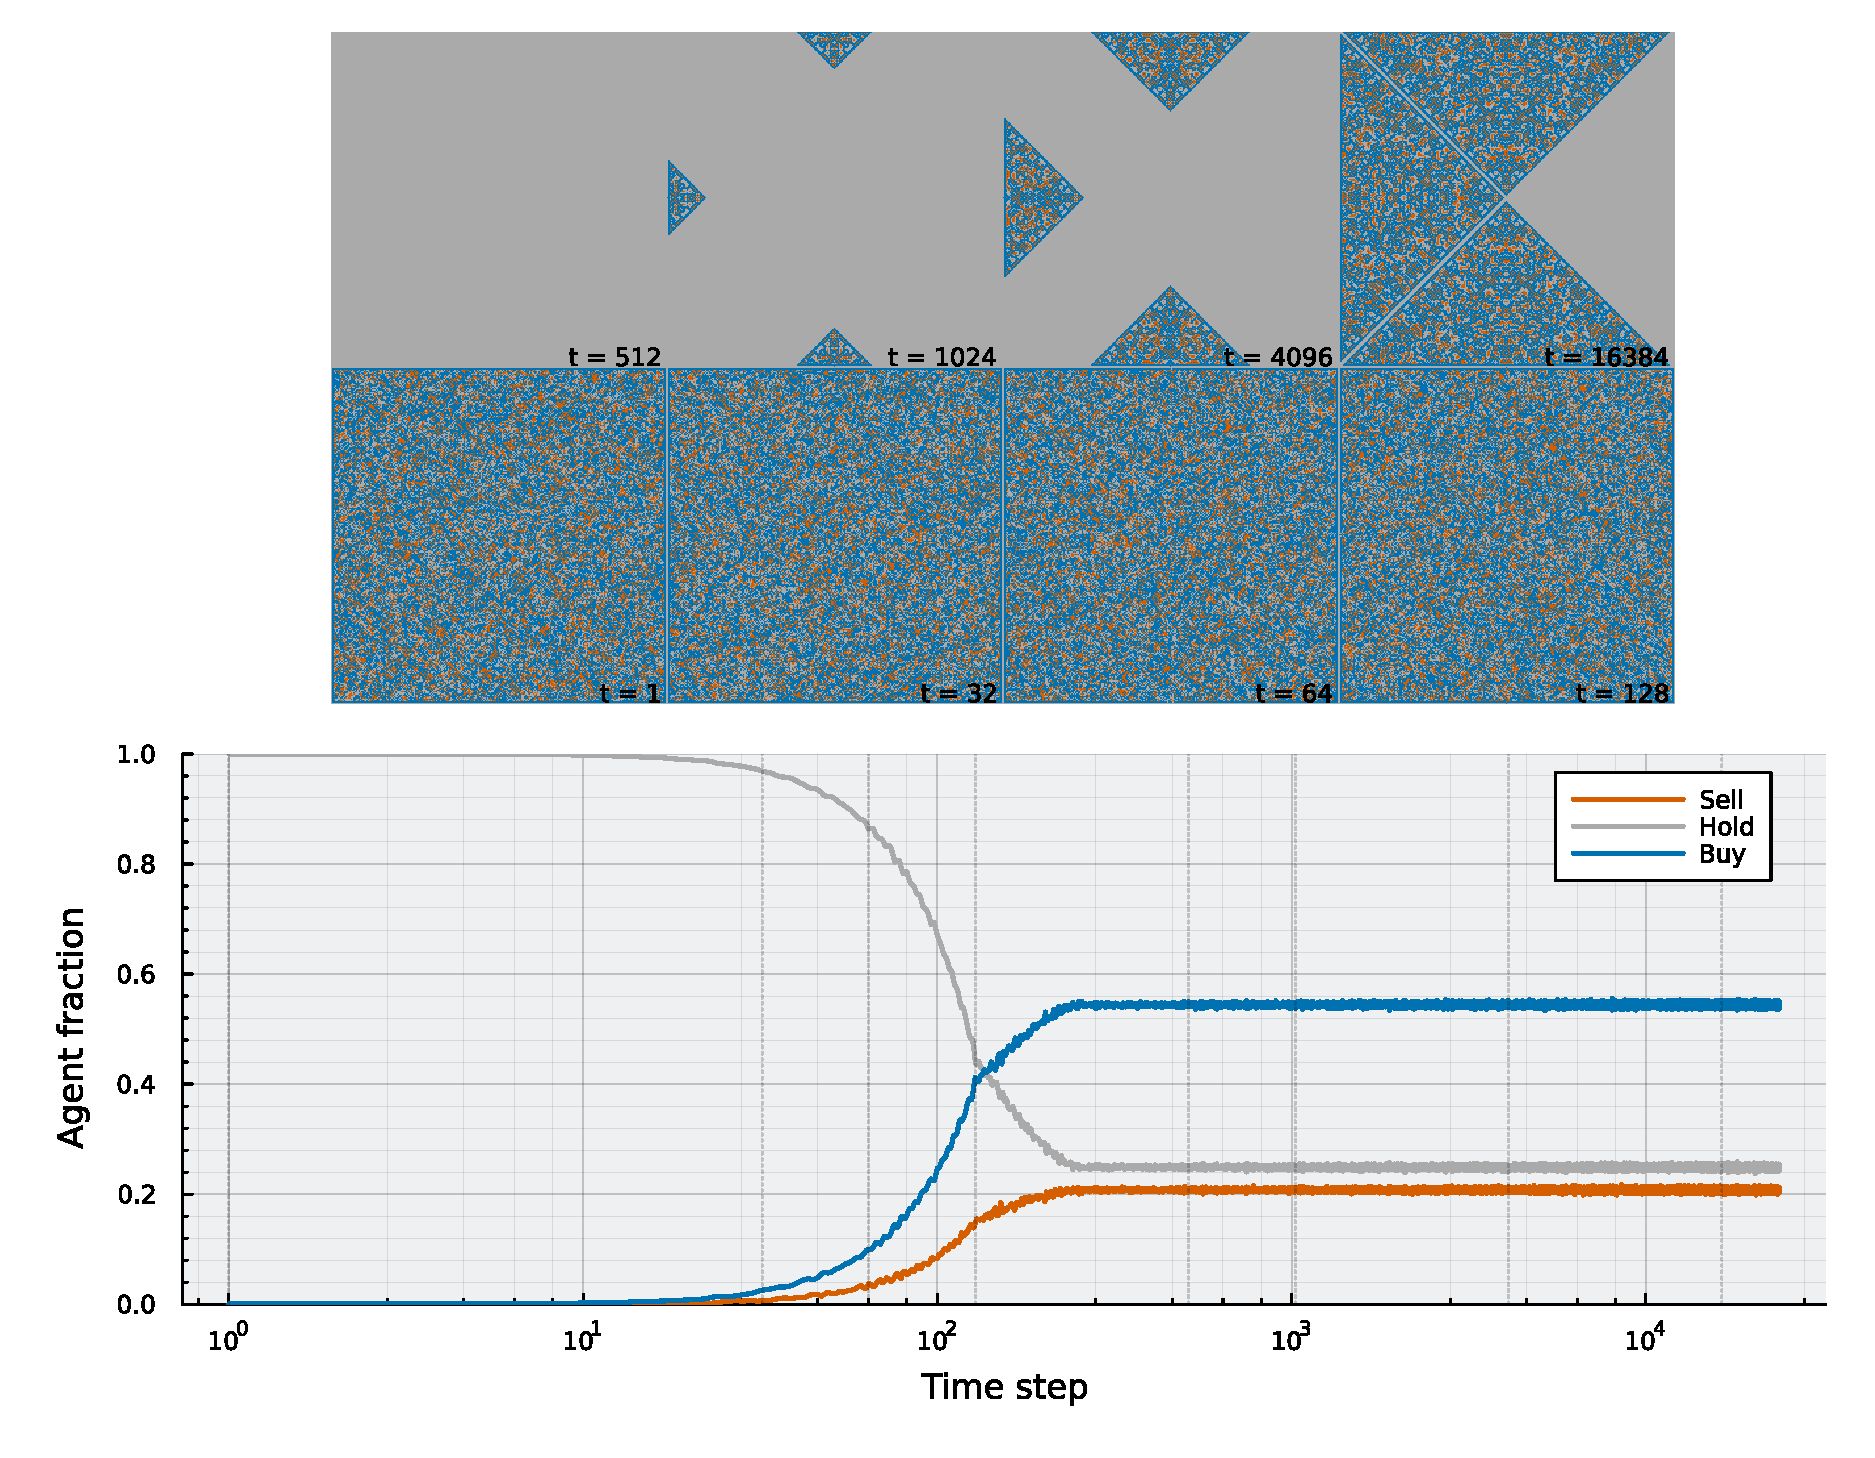
\includegraphics[width=0.95\linewidth]{figs/Fig2-Combined.pdf}
  \caption{Spatiotemporal dynamics of the $256 \times 256$ agent grid under
  Model~A (Rules~19280/19286, QQQ 2024 data). Columns share logarithmically spaced
  time points; rows vary the minority fraction~$f$. Blue = Buy, gray = Hold,
  orange = Sell. At $f = 0.15$ (middle row, $t = 8{,}236$), a sell cascade nucleates
  from a localized seed and propagates as a coherent wavefront before engulfing the grid.}
  \label{fig:fig2}
\end{figure}

\subsection{Phase Diagram}
We swept the minority fraction~$f$ from $0.0$ to $0.50$ and computed three summary
statistics---mean sell fraction, peak sell fraction, and crash frequency---for each run
(Figure~\ref{fig:fig3}). All three order parameters exhibited a sharp discontinuous
transition at a critical threshold $f_c \approx 0.145$ (dashed vertical line).

Below $f_c$, the system remained stable: the mean sell fraction hovered near $0.26$
(close to the $1/3$ expected for a uniform random mixture of three states), the peak sell
fraction never exceeded $0.30$, and no crashes occurred. Above $f_c$, the system abruptly
entered a sell-dominated regime: the mean sell fraction jumped to ${\sim}0.50$ at
$f = 0.15$ and saturated near $0.91$ by $f = 0.20$; crash frequency exceeded 95\%
(Figure~\ref{fig:fig3}C). The transition width was less than $\Delta f = 0.01$, and the
jump in the order parameter was discontinuous, both hallmarks of a first-order phase
transition rather than the smooth crossover that would characterize a second-order
(Ising-type) critical point.

These results suggest a clear economic interpretation: a small minority of contrarian
agents was harmless, because Rule~19280 (majority) agents damped local sell signals
through herding toward the dominant state. But once the contrarian fraction
exceeded~$f_c$, Rule~19286 agents were numerous enough to nucleate sell clusters that the
majority-rule agents could no longer absorb; instead, the herding mechanism
\emph{amplified} the cascade, because the local majority had tipped from buy to sell. The
result was a coordination failure---a flash crash triggered by the interaction between two
deterministic rules, without any stochastic component, learning, or adaptive strategy
switching. The crash was an emergent property of the rule mixture, not of any individual
rule.

\begin{figure}[tb]
  \centering
  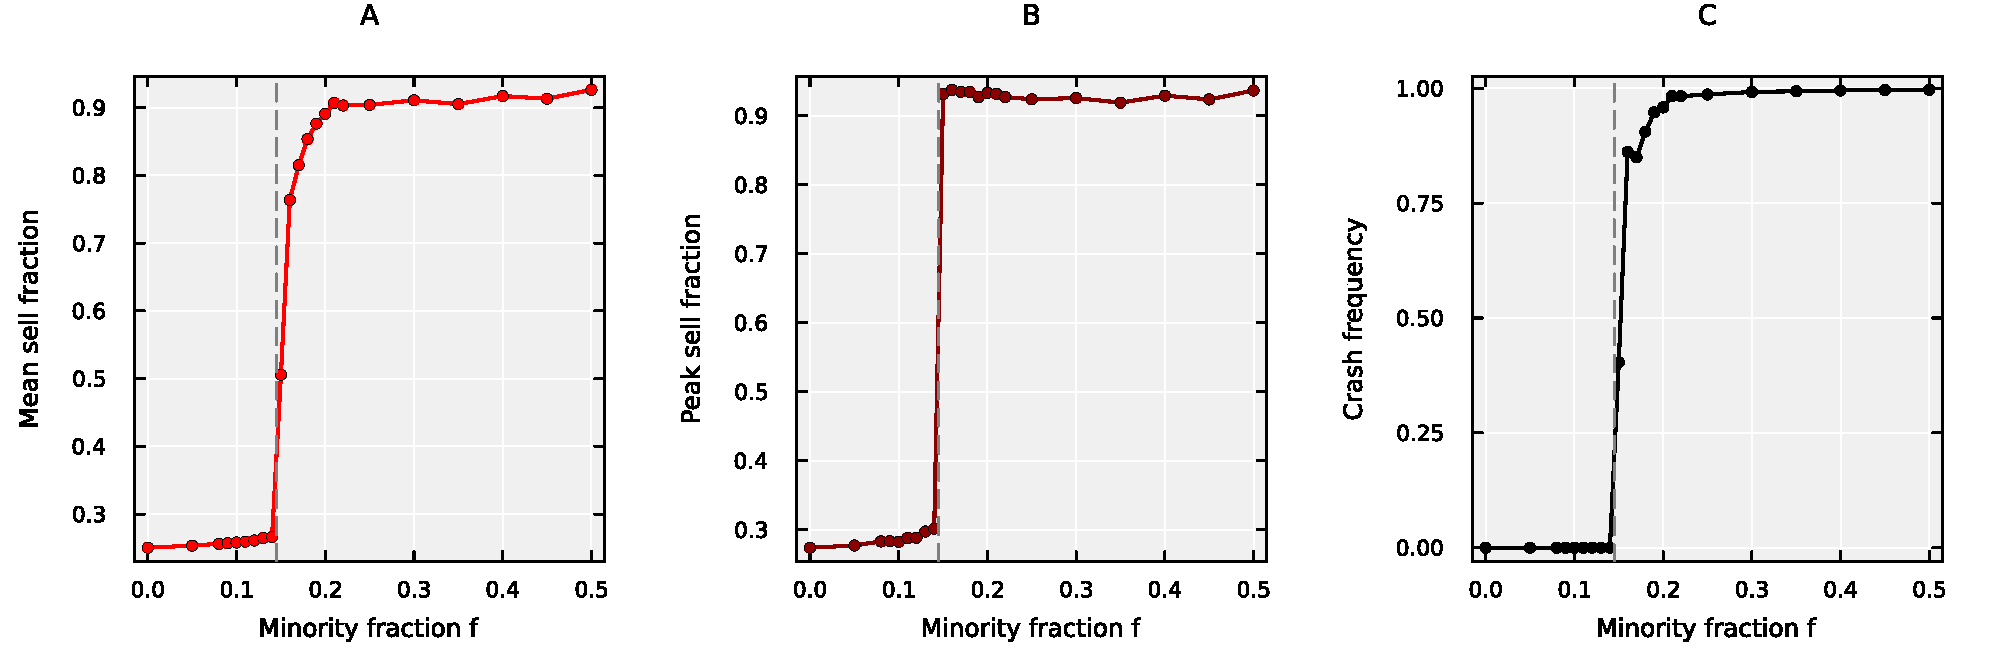
\includegraphics[width=0.95\linewidth]{figs/Fig3-PhaseDiagram.pdf}
  \caption{Phase diagram for Model~A (Rules~19280/19286, $128 \times 128$ grid).
  \textbf{A:}~Mean sell fraction vs.\ minority fraction~$f$.
  \textbf{B:}~Peak sell fraction.
  \textbf{C:}~Crash frequency (fraction of time steps with sell fraction $> 0.50$).
  Dashed vertical line marks $f_c \approx 0.145$. The transition is discontinuous,
  consistent with a first-order phase transition.}
  \label{fig:fig3}
\end{figure}


% ============================================================================
\section{Conclusion}
\label{sec:conclusion}
% ============================================================================

We presented a minimal agent-based model of financial markets in which traders on a
two-dimensional grid follow deterministic Wolfram totalistic cellular automaton rules.
The model required only two ingredients---a majority/herding rule (19280) and a
contrarian/destabilizer rule (19286)---and a single control parameter, the minority agent
fraction~$f$. We observed a sharp first-order phase transition at $f_c \approx 0.145$:
below this threshold the market remained stable; above it, the system abruptly locked
into a sell-dominated regime (Figure~\ref{fig:fig3}).

Three features distinguished this framework from prior ABMs and lattice models. First,
the CA enforced strictly local information propagation, which produced spatially resolved
sell cascades that nucleated from localized seeds and spread as coherent wavefronts
(Figure~\ref{fig:fig2}). This mechanism---a crash with a spatial history, arriving at
different parts of the grid at different times---was absent in mean-field models and
highlighted the role of spatial topology in crash formation. Second, the transition was
discontinuous, occurring over $\Delta f < 0.01$, which places it squarely within the
tipping-point framework of Scheffer et al.~\cite{scheffer2009early} and suggests that
early-warning signals (rising autocorrelation and variance) may be detectable in the
pre-transition regime. Third, the full rule space is finite and enumerable
($3^9 = 19{,}683$ rules), enabling systematic screening of agent behaviors---a property
unavailable in models with continuous behavioral parameters.

\paragraph{Limitations.}
The present study uses a single price series (QQQ, 2024 calendar year) for Model~A
validation; robustness across instruments and market regimes remains to be established.
The CA rules are deterministic and do not incorporate stochastic noise, learning, or
adaptive strategy switching---features that are present in real markets and that would
enrich the model at the cost of breaking the enumerability of the rule space. The economic
interpretation of individual rules (e.g., why a specific digit in the base-3 encoding
corresponds to contrarian behavior) remains heuristic rather than derived from utility
maximization or observed trader behavior.

\paragraph{Future directions.}
Model~B (closed-loop endogenous price) remains to be fully characterized. Its
four-dimensional parameter space $(k, w, \lambda, f)$ admits an analytical stability
analysis via mean-field linearization that may yield a closed-form expression for the
phase boundary. A key open question is whether Model~B self-organizes to criticality
without fine-tuning of~$f$---i.e., whether the reflexive feedback loop drives the system
toward its own tipping point, a phenomenon that would connect this framework to the broader
literature on self-organized criticality in financial
markets~\cite{sornette2017why,bak1987selforganized,gabaix2003theory}.


% ============================================================================
\section*{Acknowledgments}
% ============================================================================
TODO: Acknowledgments here.

\bibliographystyle{unsrtnat}
\bibliography{References_v1}

\newpage
\appendix
\section{Supplementary Material}
\label{app:supplement}

TODO: Write appendix content here.

\end{document}
